\subsection{Innlogging}
\begin{figure}[ht!]
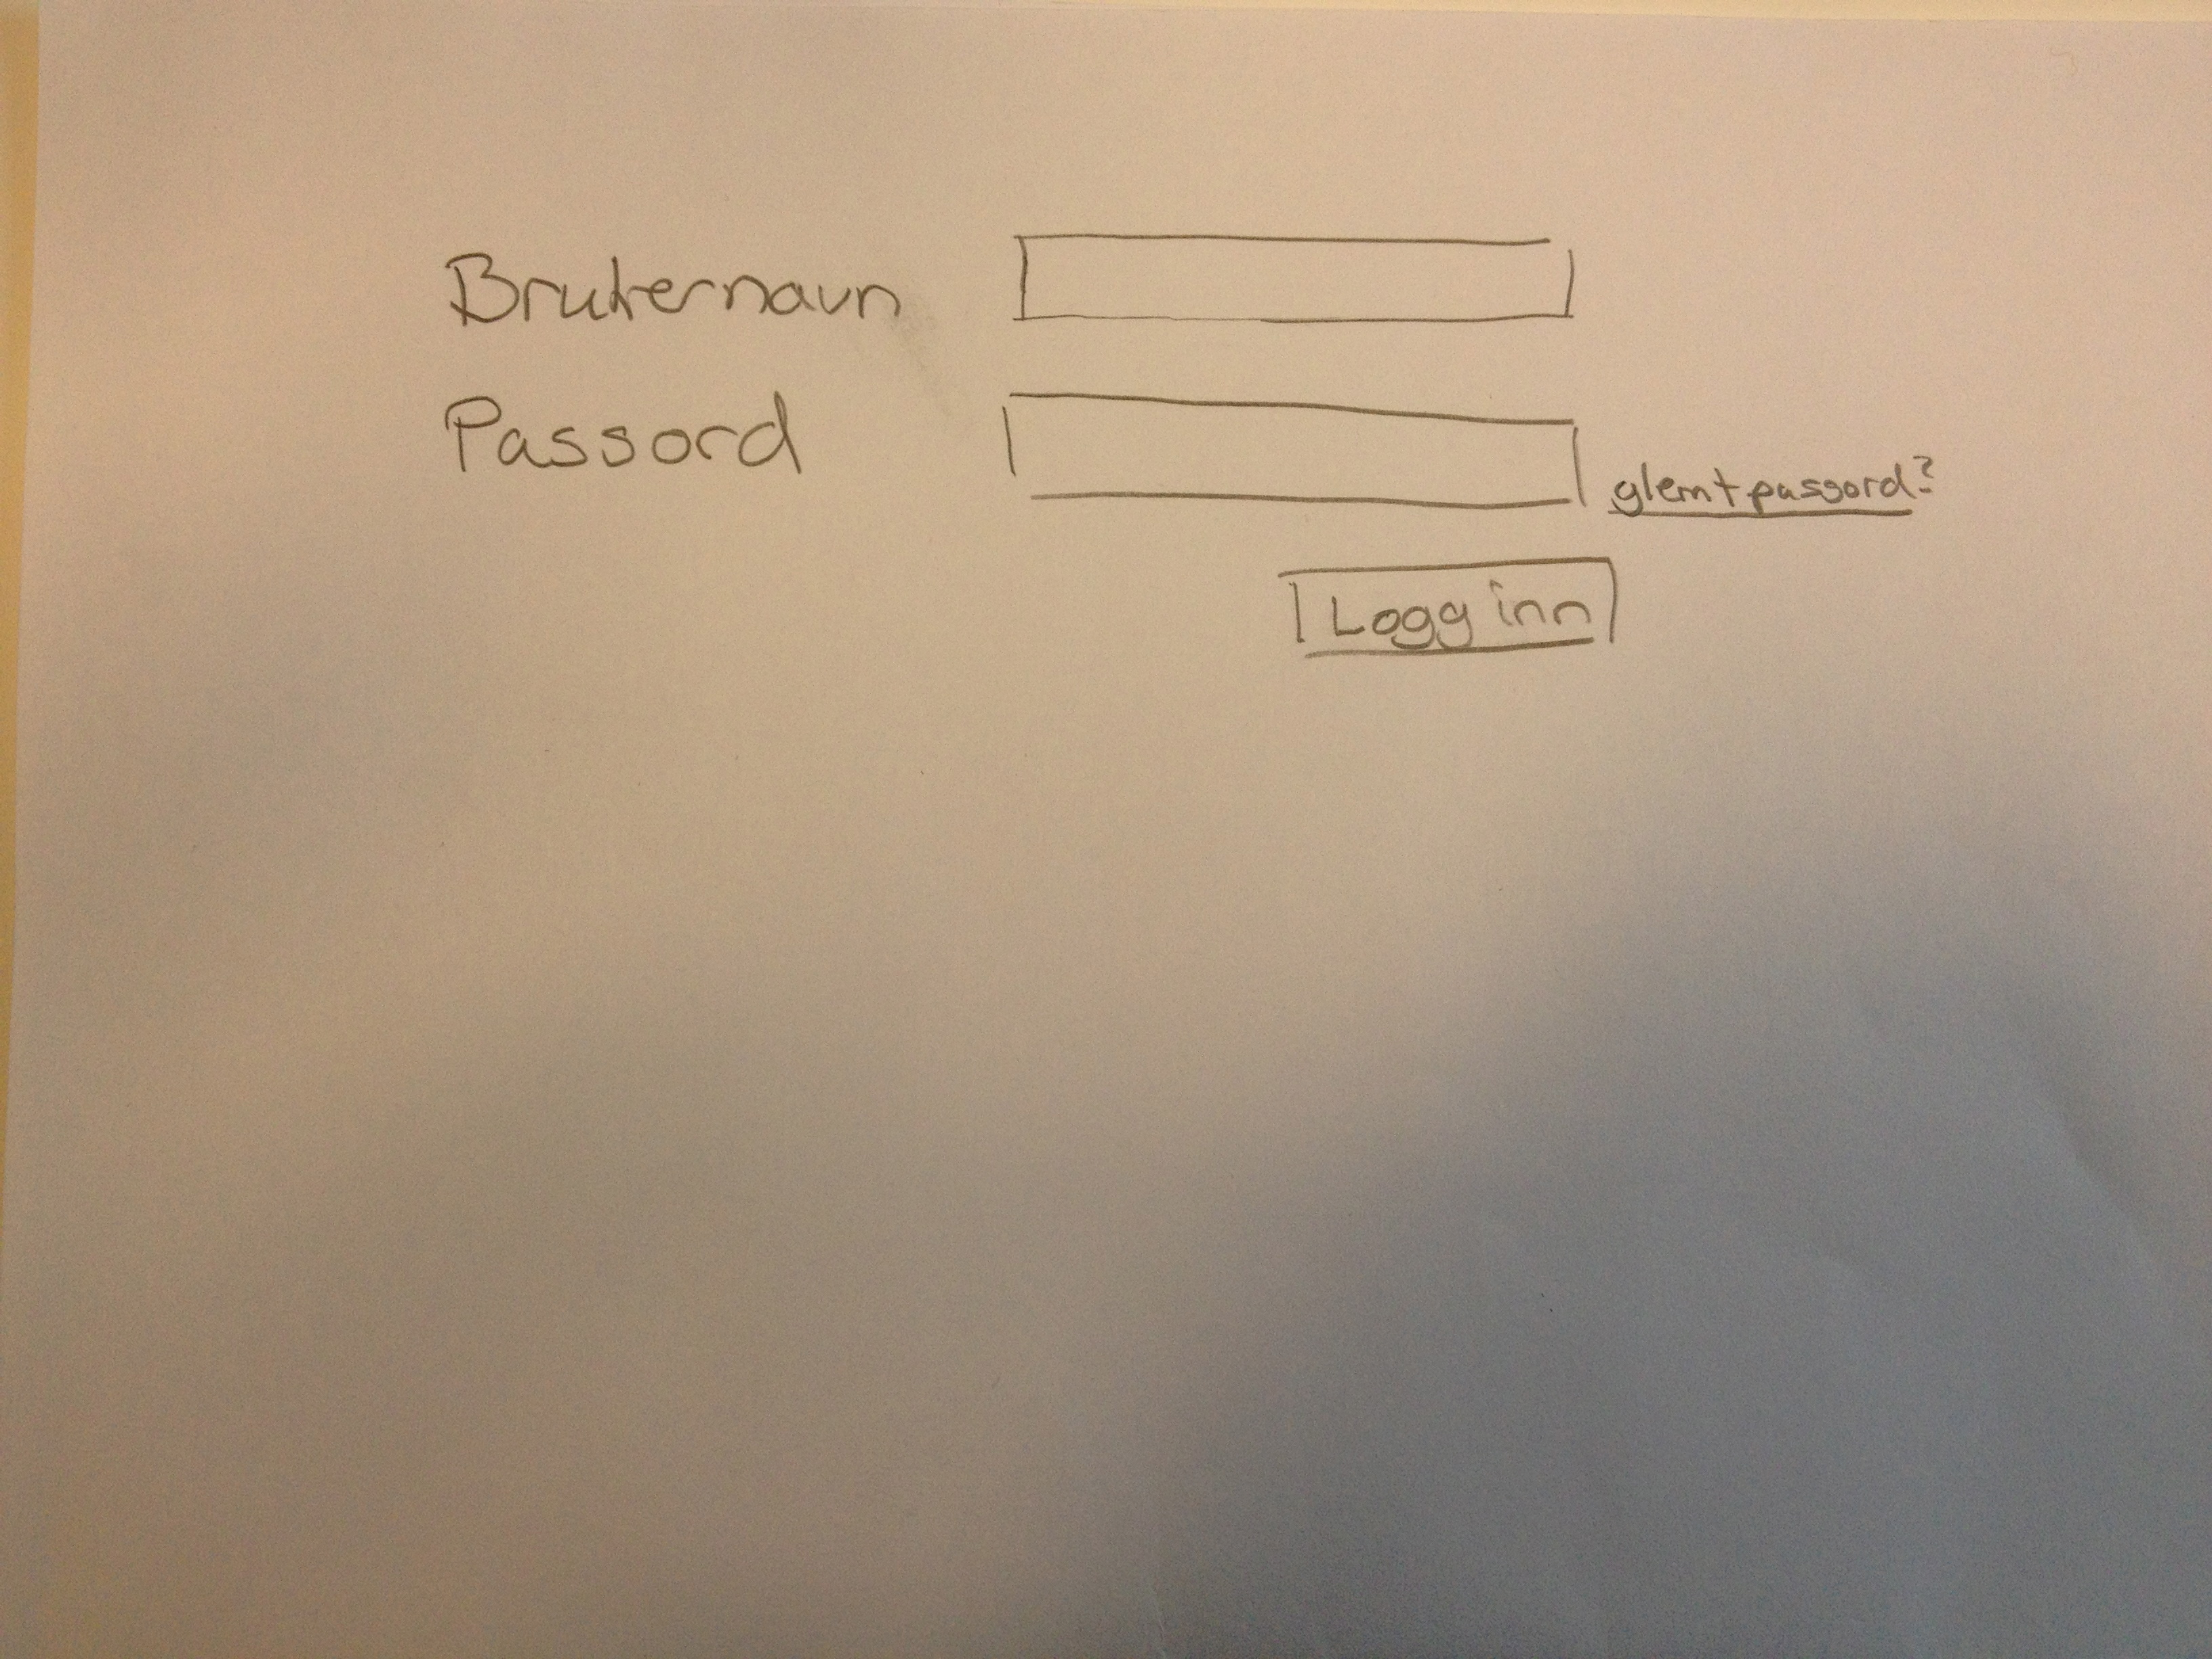
\includegraphics[width=90mm]{fig1.jpg}
\caption{Innloggings vindu}
\end{figure}
En helt enkelt innlogging skjerm der brukeren kan skrive brukernavn og passord. Vi kan også benytte “glemt passord” som tar oss til fig2. Dersom brukeren skriver feil navn eller passord, så vil det skrives ut: “feil passord og/eller brukernavn”. Dersom bruker skriver riktig informasjon, så vil han bli tatt til fig3.
\newpage

\subsection{Glemt passord}
\begin{figure}[ht!]
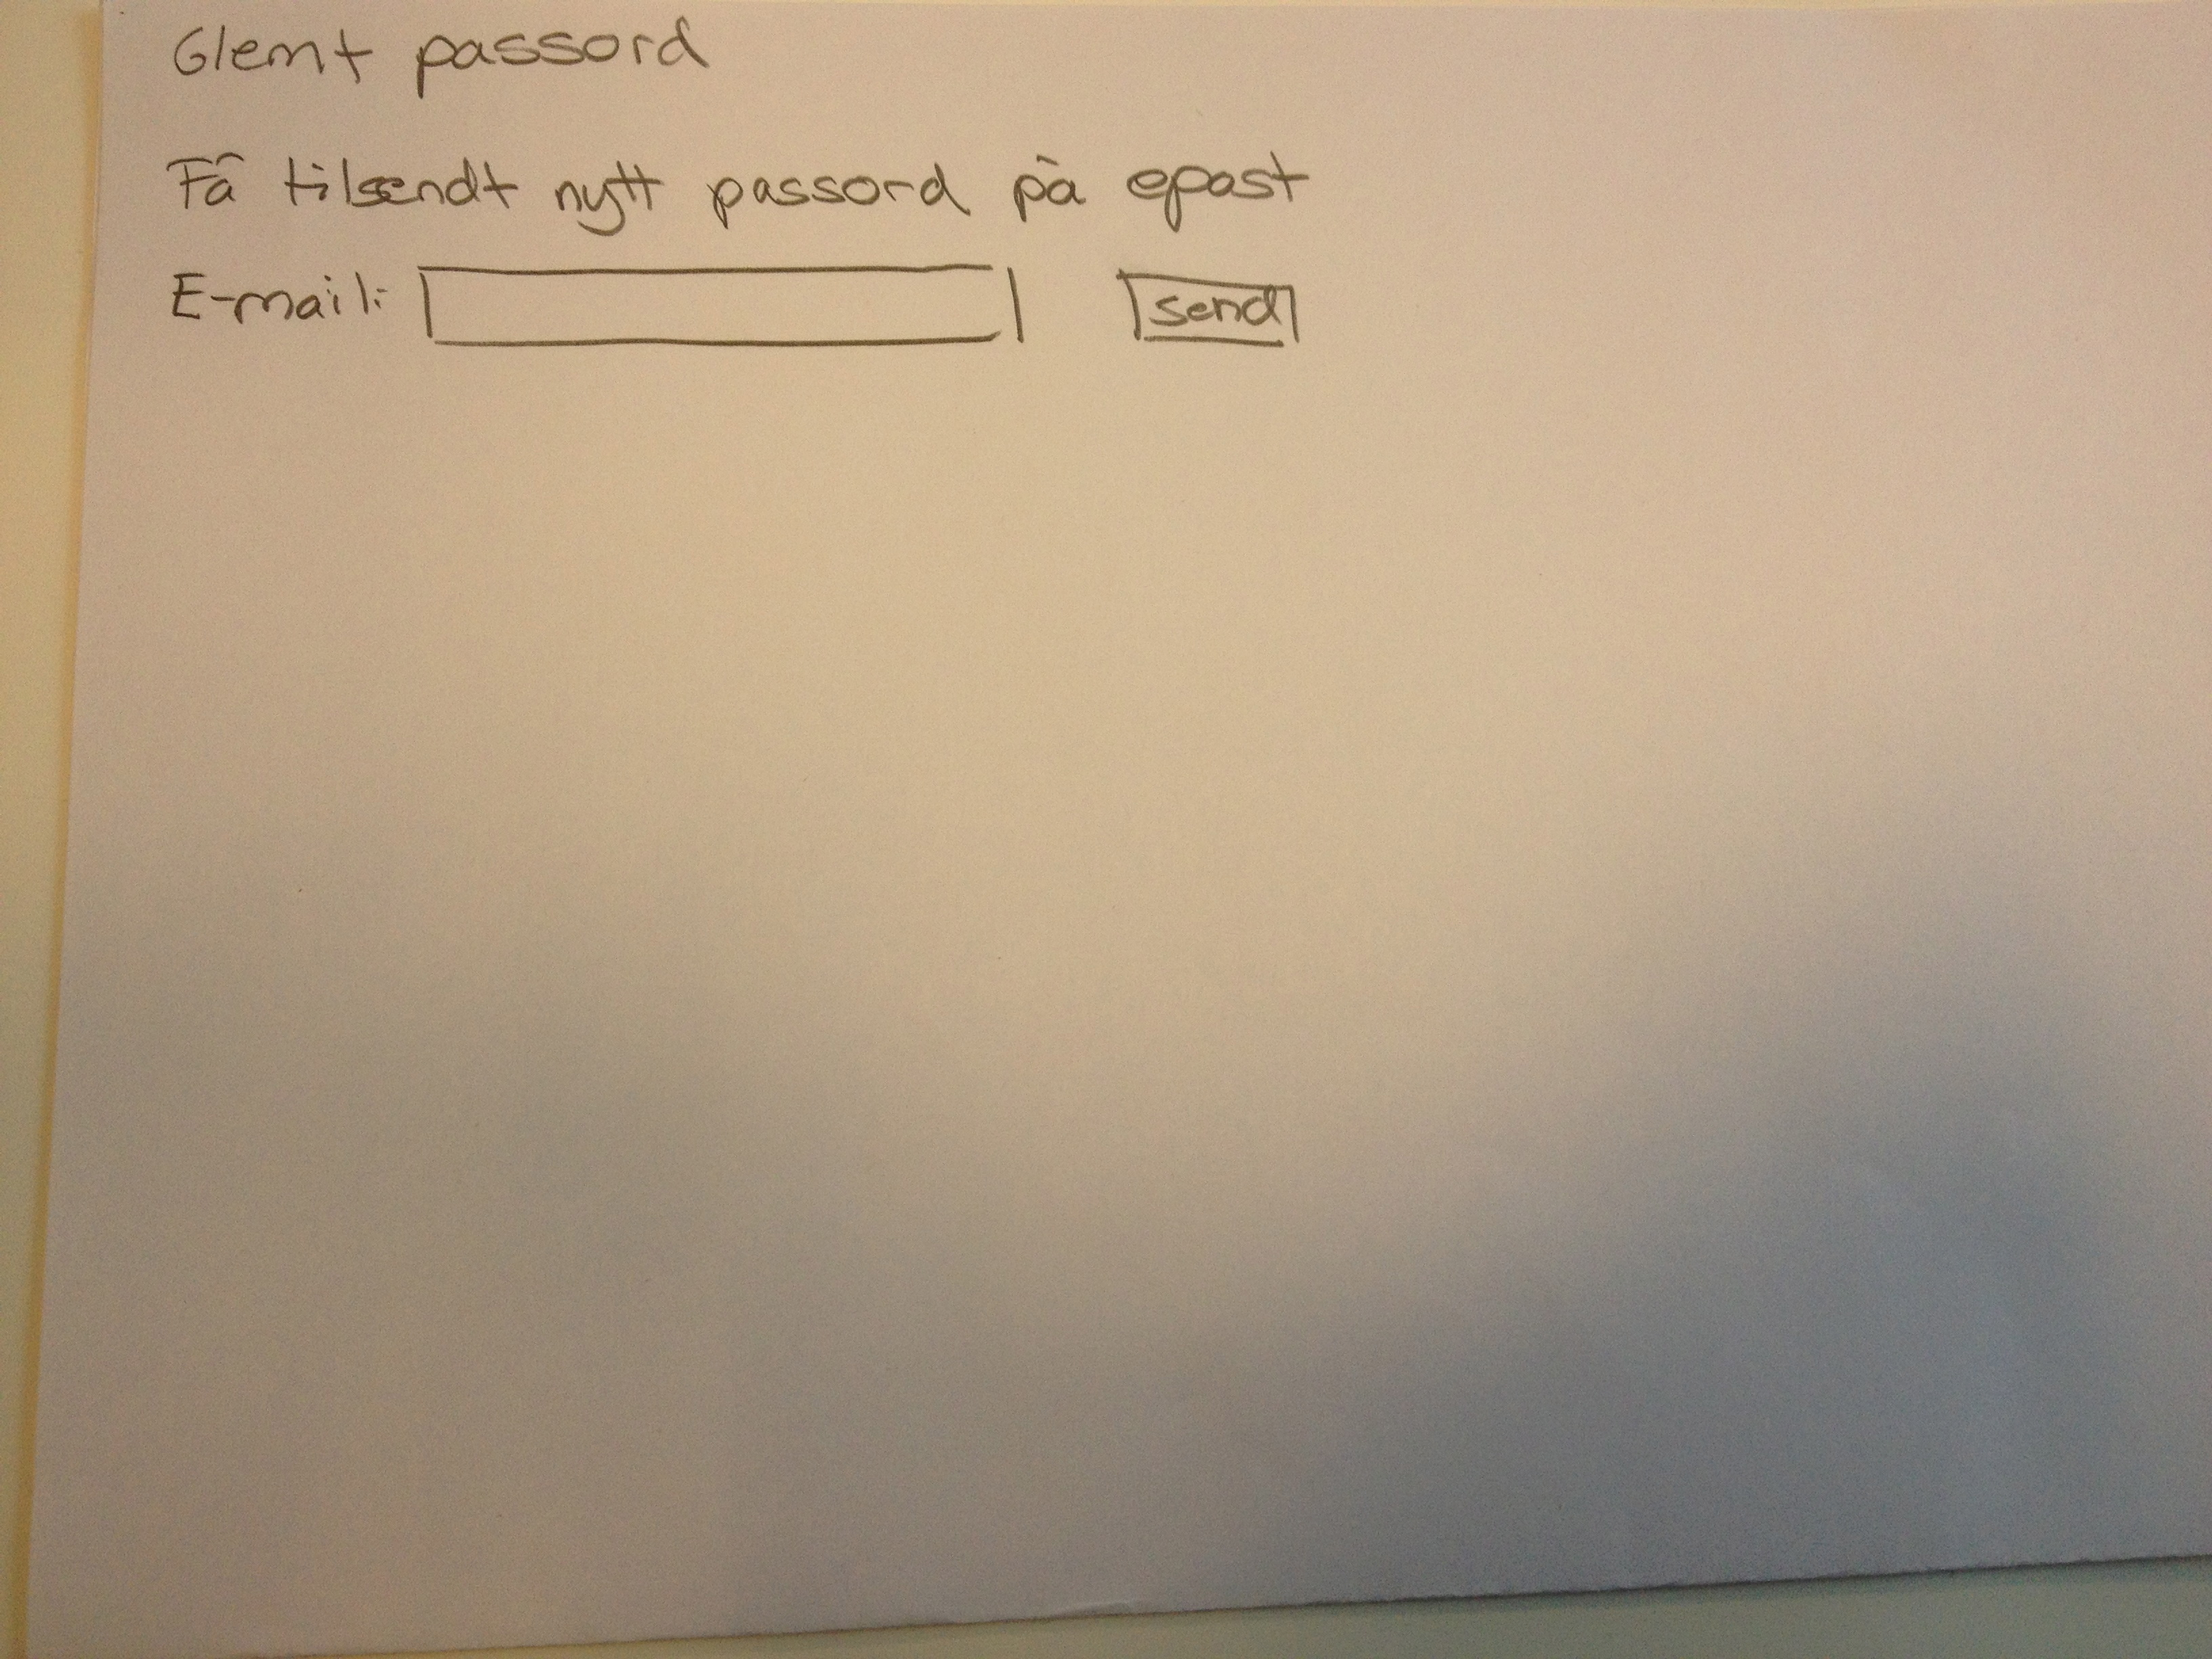
\includegraphics[width=90mm]{fig2.jpg}
\caption{glemt passord skjerm}
Et ny vindu som popper opp, her skriver man e-mail/brukernavn, avhengig av hva firma X bruker, så får de tilsendt sitt passord til sin e-mail.
\end{figure}

\newpage

\subsection{Kalendervisning}
\begin{figure}[ht!]
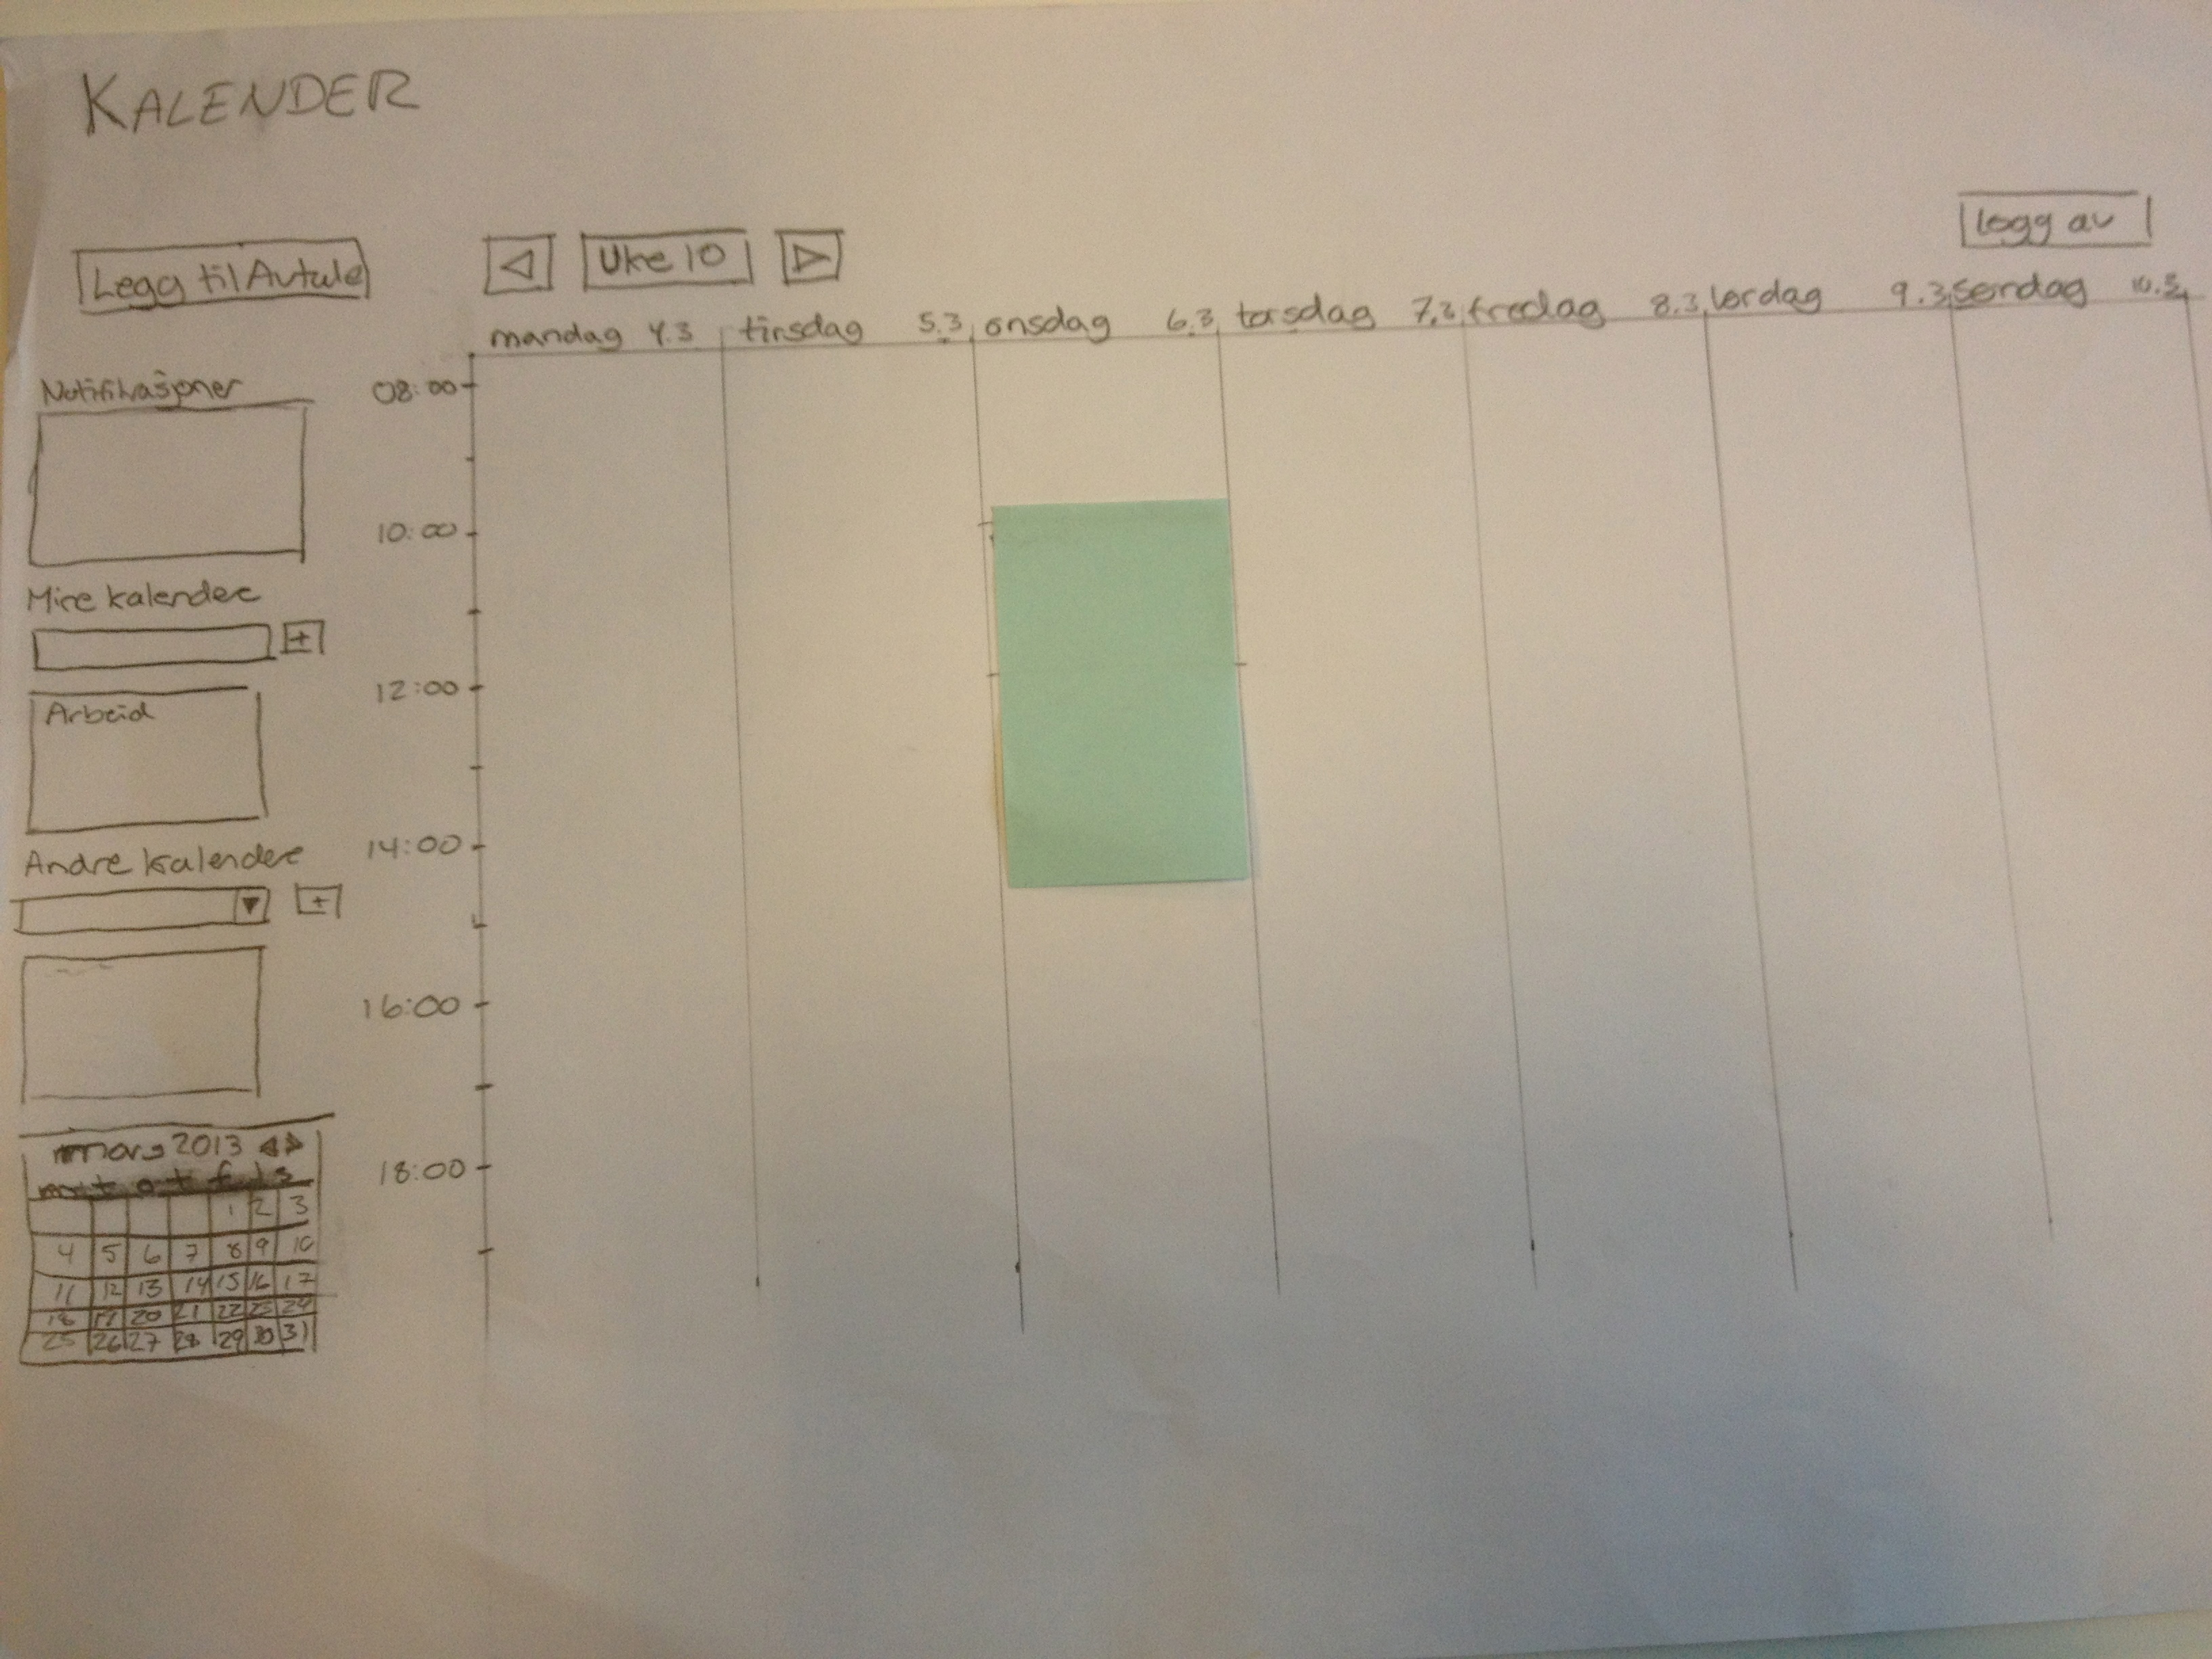
\includegraphics[width=100mm]{fig3.jpg}
\caption{Kalendervisning}
\end{figure}
Her er selve ukedagkalenderen. Man ser at på venstre side av figuren så har man flere valgmuligheter, blant annet notifikasjonsvindu. Man kan se forskjellige notifikasjoner til møter som brukeren ikke har svart på. Dersom man blir invitert til et møte, så dukker det opp en melding i vinduet, og man får muligheten til å trykke på den og fig7 dukker opp. 

Under der er det en liste av andre kalendere som brukeren kan lage selv. Man trykker på feltet og skriver hva man vil kalle kalenderen. Under der igjen så har vi de andre sine kalendere, vi tenkte at man skal kunne hente andre brukere sin kalender for å lettere kunne velge ett tidspunkt som passer for flere personer til et møte. Andre brukere sine kalendere er i forskjellige farger så man lettere kan skille dem fra hverandre. Vi har også en månedskalender under for å holde styr på ukene som kommer. Vi har valgt å ta med hvilket ukenummer det er nå, siden folk ofte benytter ukenummer, og mange andre kalendersystem ikke viser det. Øverst ser vi en knapp som heter “legg til avtale”, man trykker på den for å opprette en ny avtale og kommer da til fig4. Man kan også endre på hvilken uke kalenderen skal vise, det gjør man ved hjelp av pilene ved siden av ukenummeret. Øverst i høyre hjørne er det en logg av knapp, som logger brukeren av systemet.

\newpage

\subsection{Oppretting av møte}
\begin{figure}[ht!]
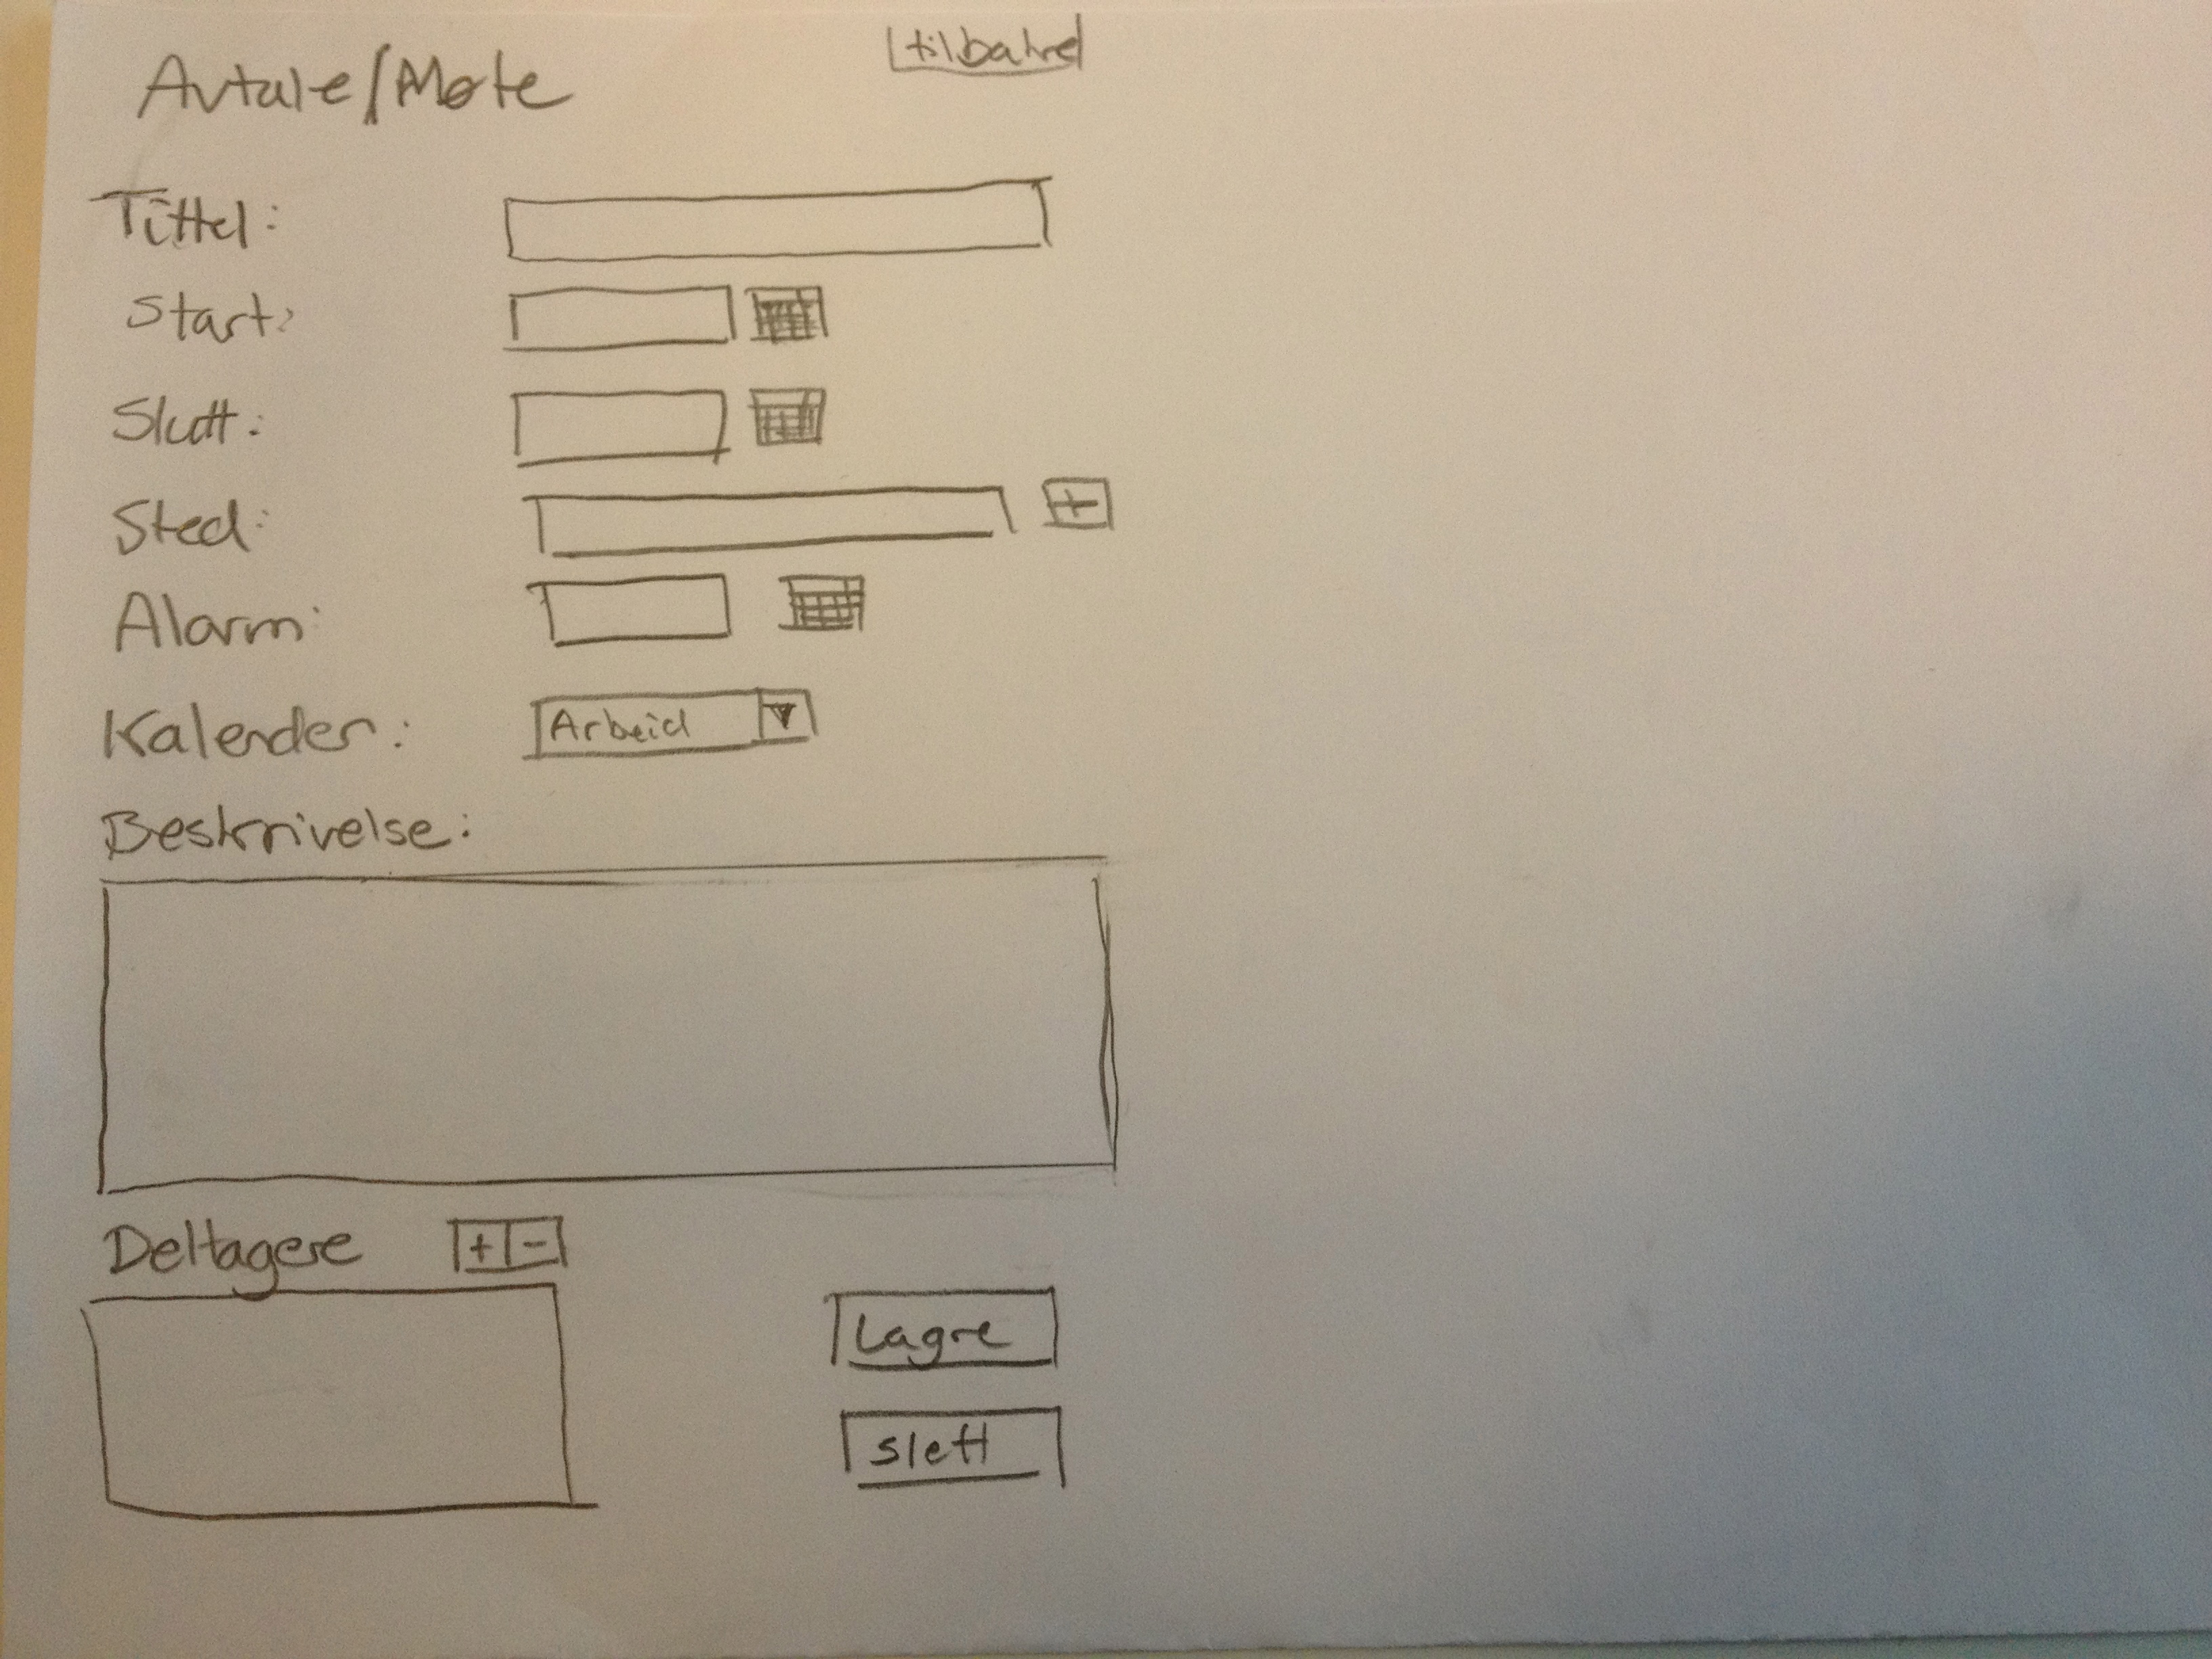
\includegraphics[width=90mm]{fig4.jpg}
\caption{Laging av møteinnkalling og avtale}
Her kan man opprette avtale, alle feltene skal kunne fylles ut, og når man trykker på kalenderikonet ved siden av tid så dukker det opp en liten månedskalender der man kan velge hvilken dag man vil ha. I den lille kalenderen så er det også et lite felt der man kan skrive det bestemte tidspunktet. Man kan i feltet for sted skrive inn et valgfritt sted eller reservere et møterom ved å trykke på “+” knappen. Fig5 popper da opp.
Under beskrivelse kan man skrive inn en kort beskrivelse av møte/avtalen. For å legge til deltagere trykker man på  “+” knappen og fig 6 kommer opp. Mens hvis man trykker på en deltager og trykker “-”  vil den valgte personen slettes fra deltagerlisten. Så kan man enten lagre eller slette avtalen med knappene. 
\end{figure}

\newpage

\subsection{Rommbestilling}
\begin{figure}[ht!]
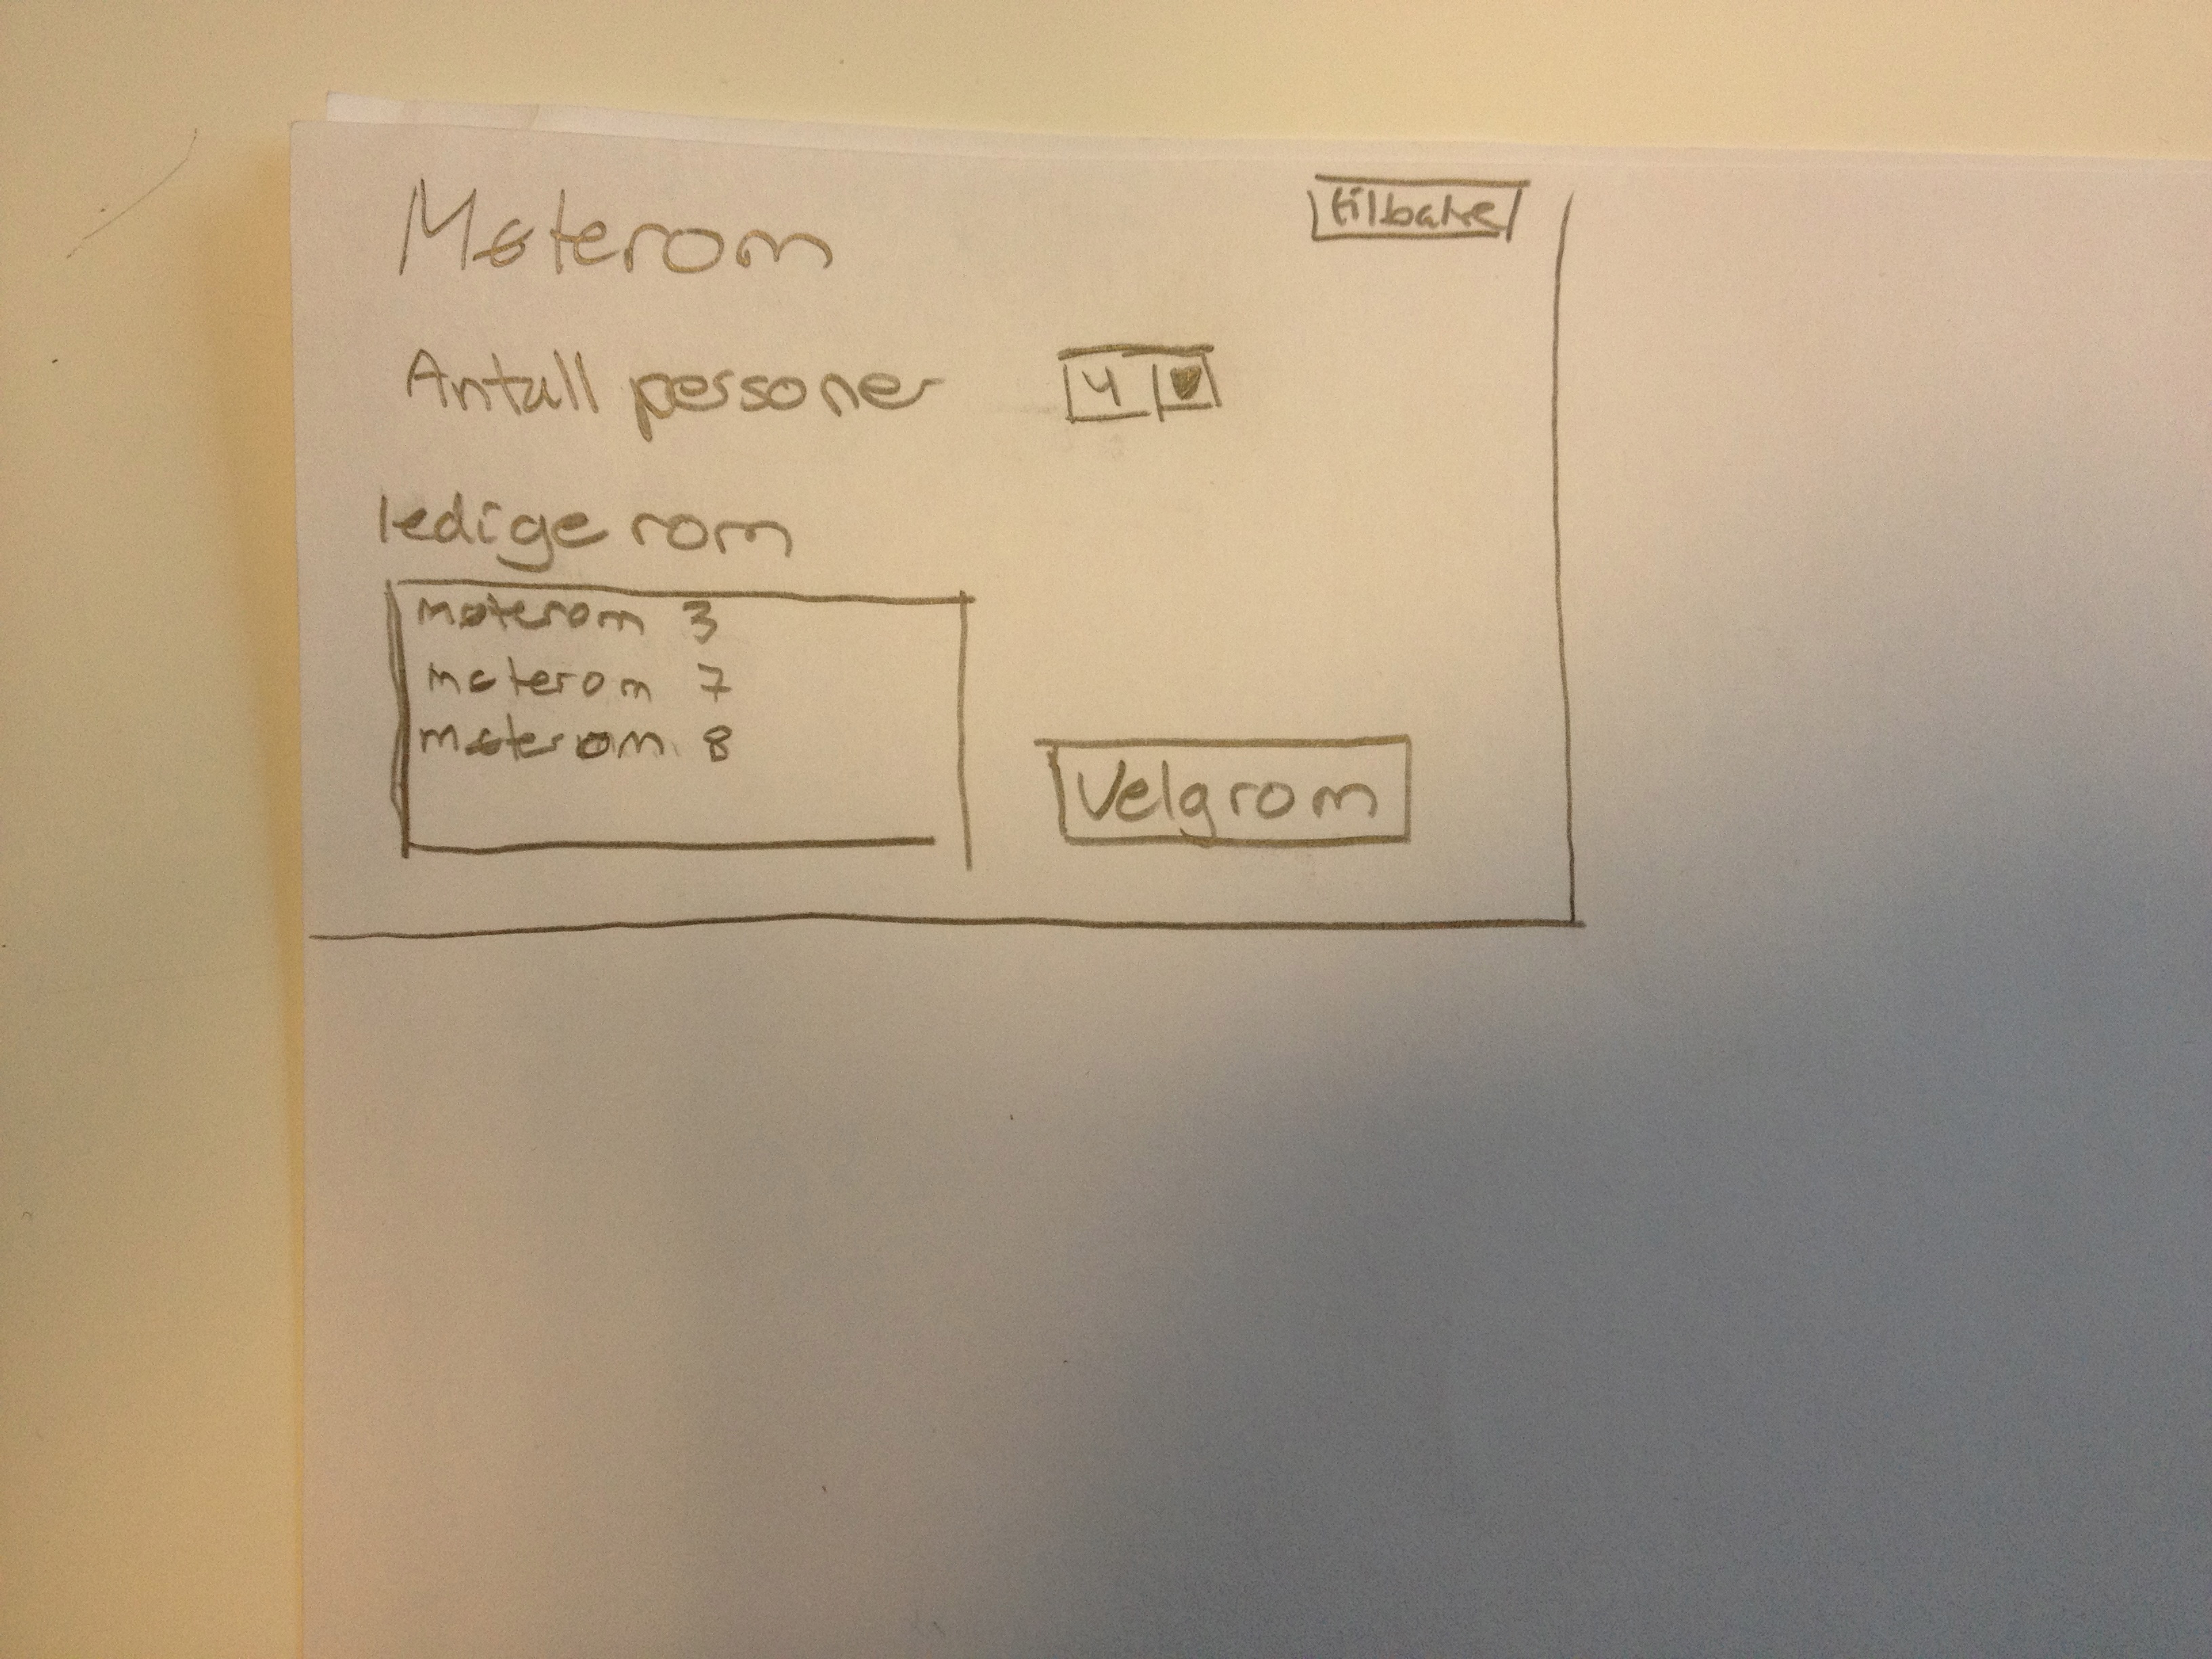
\includegraphics[width=90mm]{fig5.jpg}
\caption{Bestilling av rom}
Her har man en scroll-bar som man bruker til å velge antall personer, og en liste med ledige rom i tidsperioden avtalen er satt til. Man bekrefter valgene sine ved å trykke på “velg rom”. Dersom man trykker på “tilbake”, så vil man bli tatt tilbake til fig 3.
\end{figure}

\newpage


\subsection{Legge til deltager}
\begin{figure}[ht!]
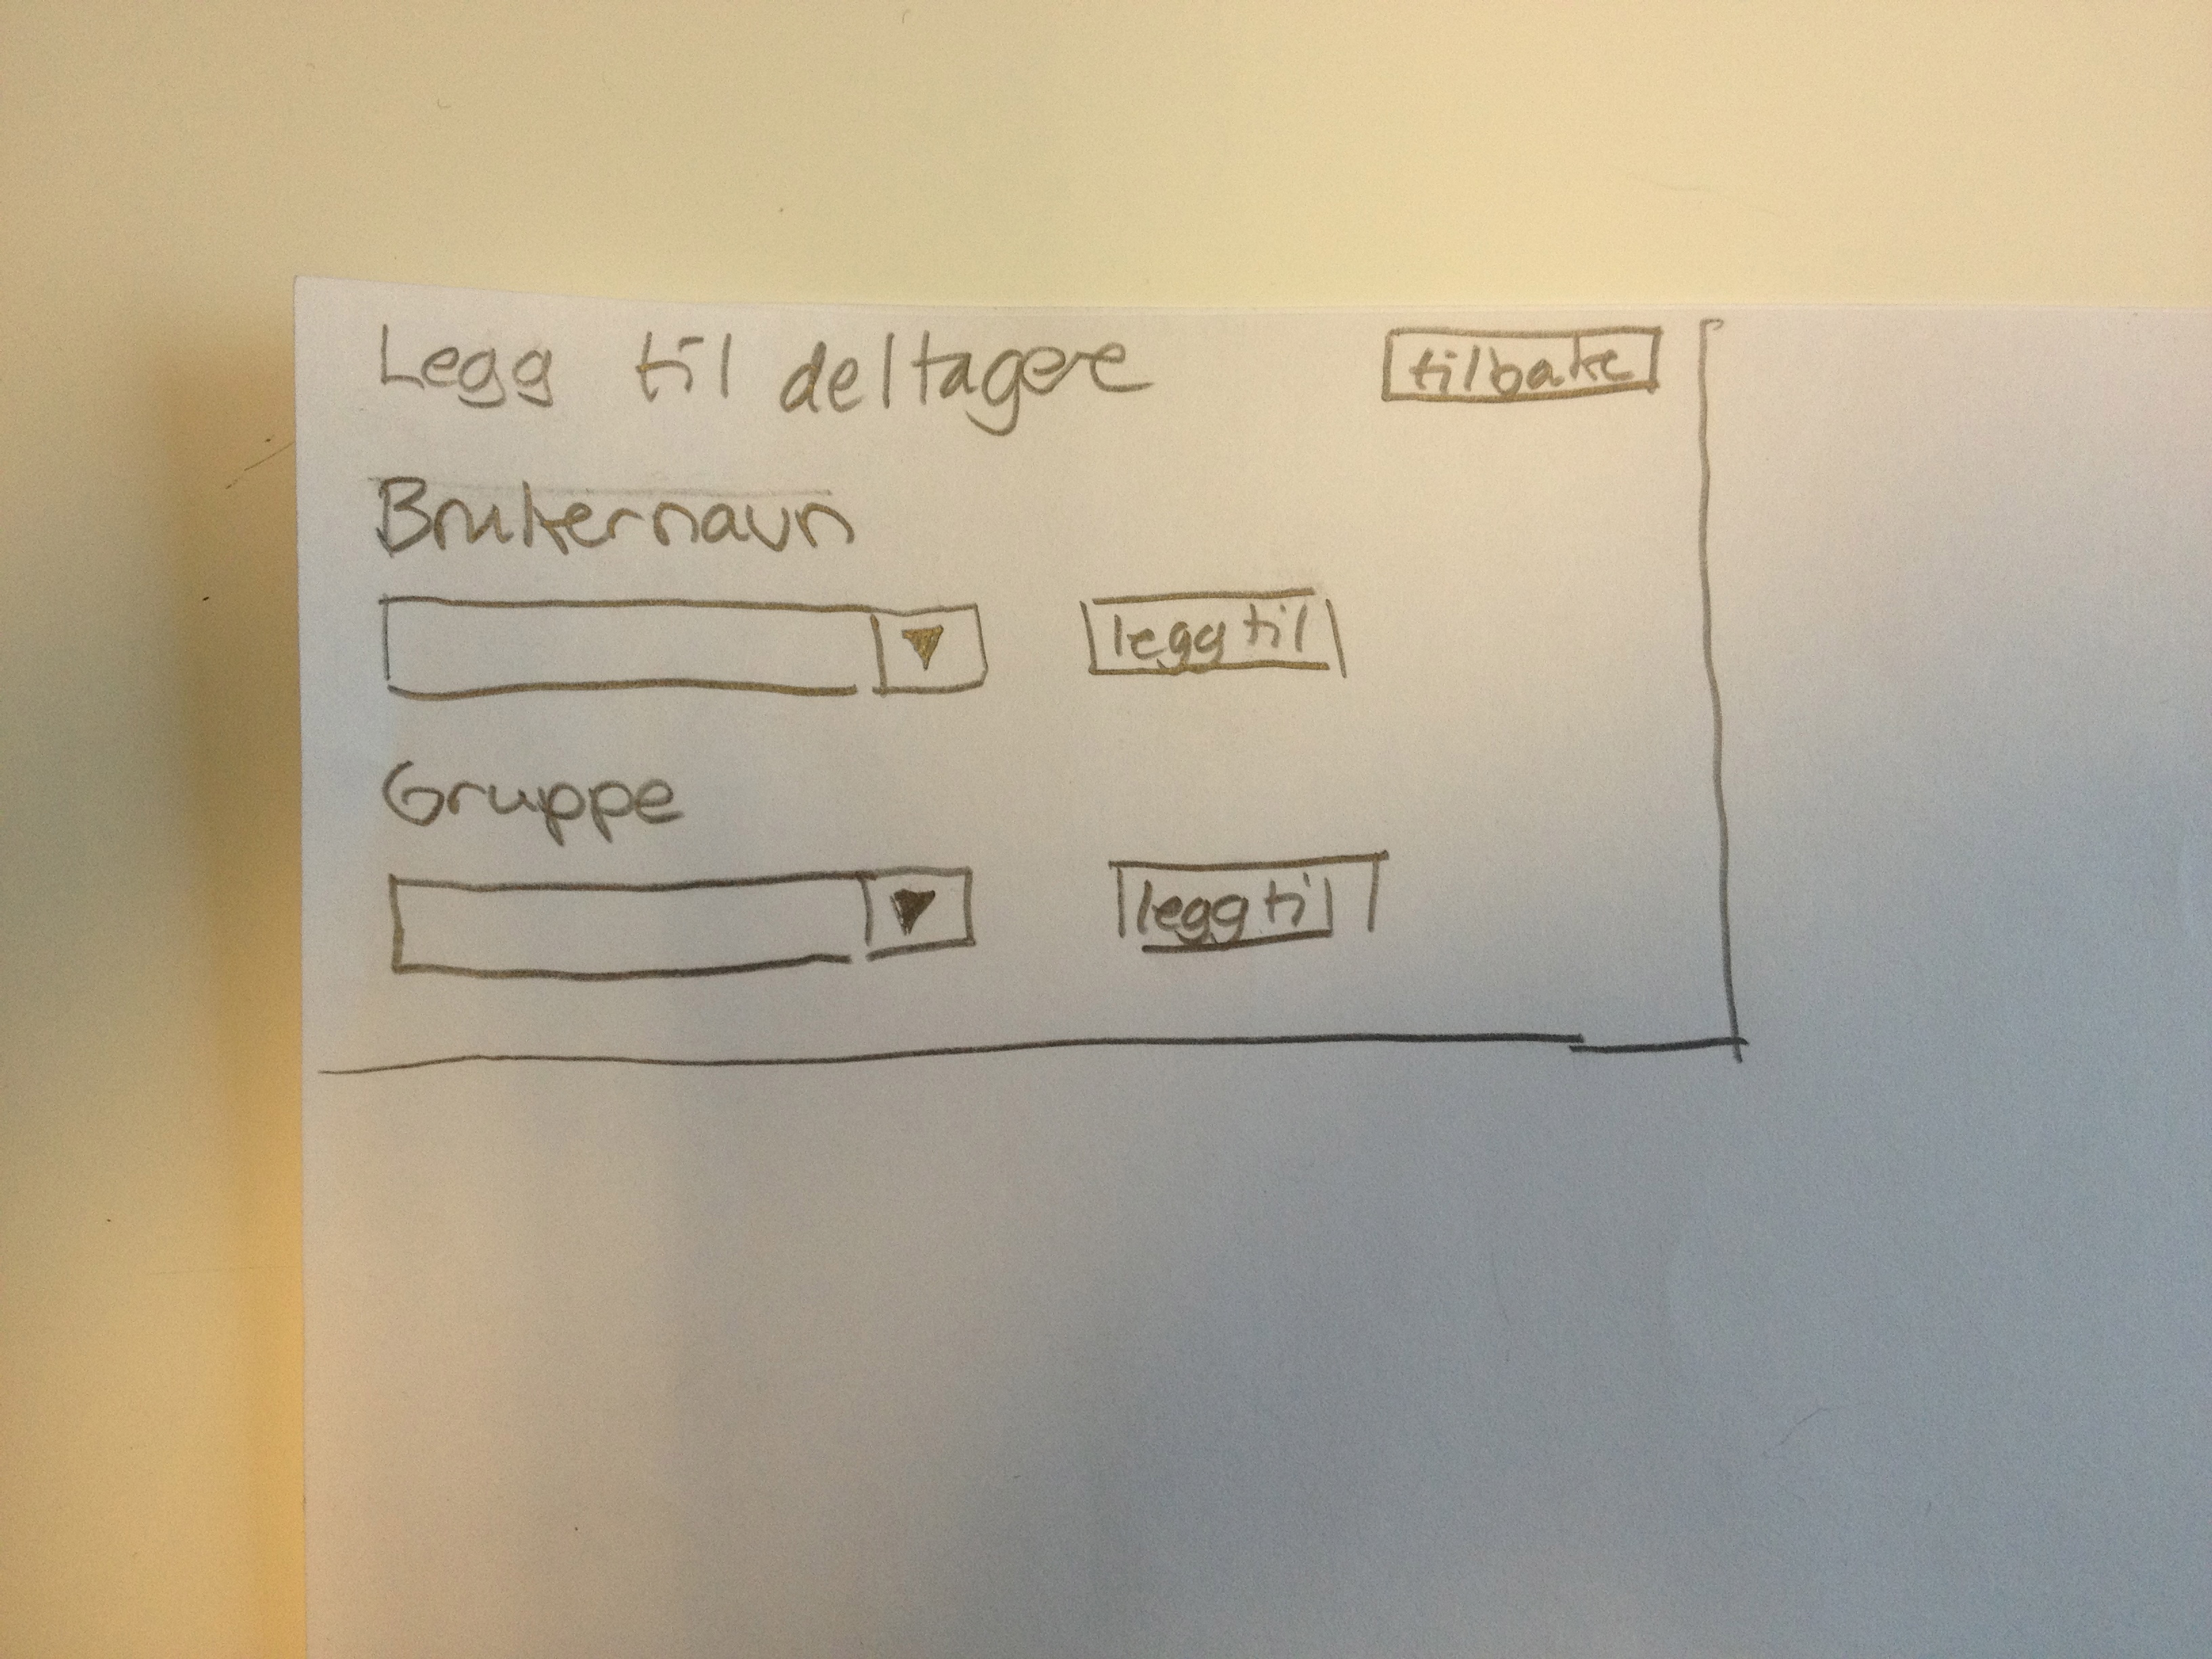
\includegraphics[width=90mm]{fig6.jpg}
\caption{ Legge til Deltager}
Her er det to felt, det ene feltet kan man skrive brukernavnet til hver bruker, pilen er for å illustrere at når man begynner å skrive navnet til en deltager, så kommer forslagene under i form av en liste. Ett av kravene var også at det skal være mulig å legge til en gruppe med personer. Dette gjøres på samme måte som når man legger til en bruker, bare ved at man skriver inn gruppenavn. Da vil alle brukerne som er lagt til i gruppen bli invitert som enkeltpersoner.
\end{figure}

\newpage
\subsection{Avtalevisning}
\begin{figure}[ht!]
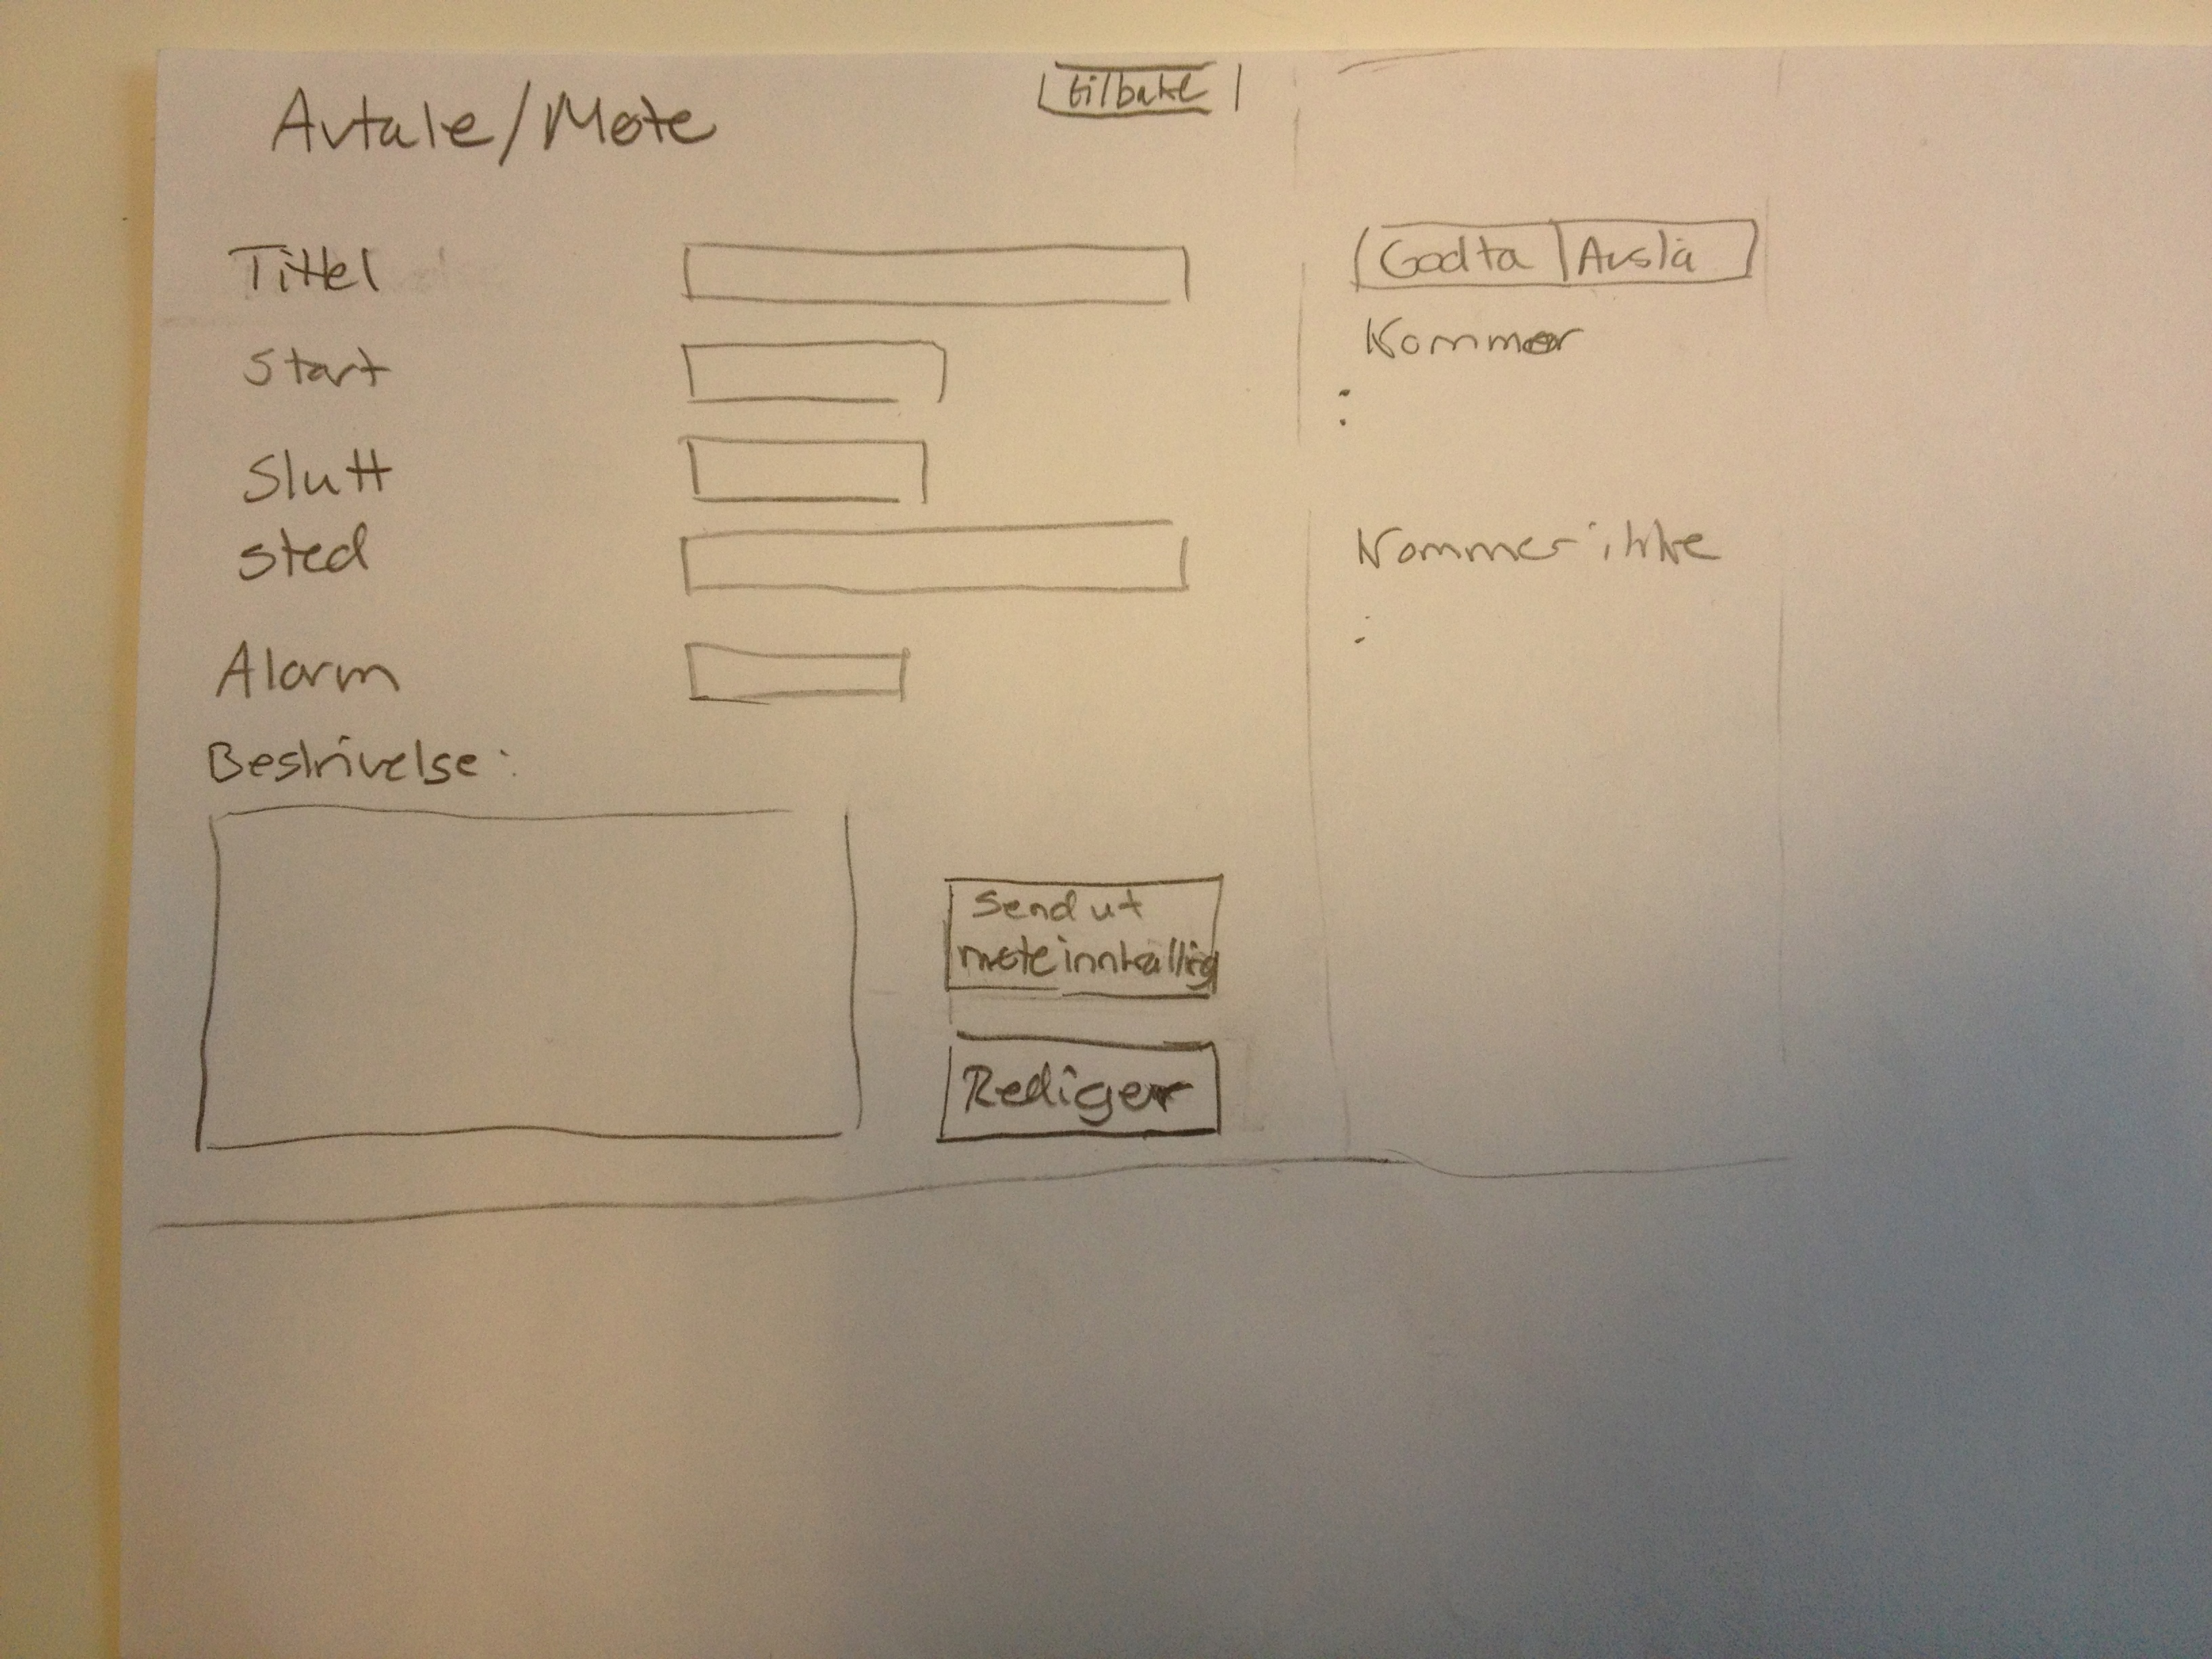
\includegraphics[width=90mm]{fig7.jpg}
\caption{Avtalevisning}
Her vises alle opplysninger angående avtalen, feltene kan ikke endres. Dersom man er møtelederen(personen som opprettet møte), har man også mulighet til å sende ut møteinnkalling. Når man har trykket på send notifikasjon, så vil alle deltagere få oppdatering når møtet blir endret. Er man møteleder har man muligheten til å endre på møte, og knappen “rediger” vil ta deg tilbake til fig4. Til høyre for figuren så ser man to mulige knapper, godta og avslå, dersom man velger en av dem, så blir den muligheten grået ut. Man kommer da på listen under, over hvem som kommer og hvem som ikke kommer. “tilbake”-knappen vil ta deg tilbake til fig3.
\end{figure}